% scopiazzato dal template di Matteo Longeri (grazie!)
%%%%%%%%%%%%%%%%%%%%%%%%%%%%%%%%%%%%%%%%%%%%%%%%%%%%%%
\documentclass[12pt,a4paper]{report}
% o article, book, ...



%%%%%%%%%%%%%%%%%%%%%%%%%%%%%%%%%%%%%%%%%%%%%%%%%%%%%%
% packages...
\usepackage[utf8]{inputenc}
\usepackage[english,italian]{babel}
\usepackage[hyphens]{url}

% Per generare il file PDF aderente alle specifiche PDF/A-1b. Verificarne poi la validità.
%\usepackage[a-1b]{pdfx}

\usepackage{hyperref}
\usepackage{graphicx}
\usepackage{url}
\usepackage{caption}

% Per inserire testo a caso in attesa di realizzare i capitoli
\usepackage{lipsum}

\usepackage{amsmath}
\usepackage{pgfplots}
\usepackage{layouts}

%%%%%%%%%%%%%%%%%%%%%%%%%%%%%%%%%%%%%%%%%%%%%%%%%%%%%
\begin{document}

% Frontespizio
\begin{titlepage}
\begin{center}

\includegraphics[width=\textwidth]{Logo.jpg}\\
{\large{\bf Corso di Laurea in Informatica}}
\end{center}
\vspace{12mm}
\begin{center}
{\huge{\bf Apprendimento di insiemi fuzzy nell'ambito del web semantico}}\\
\end{center}
\vspace{12mm}
\begin{flushleft}
{\large{\bf Relatore:}}
{\large{Prof. Dario Malchiodi}}\\
\vspace{4mm}
{\large{\bf Correlatore:}}
{\large{Prof.ssa Anna Maria Zanaboni}}\\
\end{flushleft}
\vspace{12mm}
\begin{flushright}
{\large{\bf Tesi di Laurea di:}}
{\large{Alessia Cecere}}\\
{\large{\bf Matr. 923563}}\\
\end{flushright}
\vspace{4mm}
\begin{center}
{\large{\bf Anno Accademico 2020/2021}}
\end{center}
\end{titlepage}


\tableofcontents


% o sections (dipende dal documentclass)
\chapter*{Introduzione}
\chapter{Apprendimento di insiemi fuzzy}
\section{Gli insiemi fuzzy}

Gli insiemi fuzzy sono una variante degli insiemi classici introdotta da Lotfi Zadeh del 1965, che li definisce \lq\lq una classe di oggetti con un continuo di gradi di appartenenza\rq\rq\cite{fuzzysetspaper}.

Vengono utilizzati in situazioni in cui è impossibile identificare, come avverebbe tramite un generico classificatore, una soglia univoca oltre la quale un elemento si può dire appartenente a un determinato insieme. In questi contesti è necessario dire che l'elemento appartiene all'insieme con un certo grado di intensità. Per capire meglio la differenza, immaginiamo di definire \lq\lq l'insieme dei laureati\rq\rq: preso un elemento dell'universo del discorso, è possibile definire  se è vero o falso che questo vi appartiene. Pensiamo invece, come fa Zadeh, a una \lq\lq classe degli uomini alti\rq\rq\cite{fuzzysetspaper}, o alla \lq\lq classe dei caffè dolci\rq\rq;  si tratta di insiemi di carattere più qualitativo: non tutti gli elementi vi appartengono allo stesso modo.  Il concetto di \emph{membership degree} è formalizzato tramite la funzione di appartenenza all'insieme fuzzy $f: X \mapsto [0,1]$, generalizzazione della funzione booleana classica $f: X \mapsto \{0,1\}$;  $f(x) = 1 $ indica totale appartenenza all'insieme, $f(x) = 0 $ totale non-appartenenza, con i valori intermedi dell'intervallo ad esprimere il grado di appartenenza.
In questo modo un elemento può appartenere a più insiemi che esprimono caratteristiche opposte (ad esempio \lq\lq l'insieme delle persone vecchie\rq\rq e \lq\lq l'insieme delle persone giovani\rq\rq\cite{fuzzysystemspaper}) con gradi differenti, e questo concorre a far sì che gli insiemi fuzzy giochino un ruolo importante in contesti di informazione incerta, aggiugendo un potere descrittivo enorme.
Tramite principio di estensione, Zadeh riesce ad applicare agli insiemi fuzzy qualunque operazione tipica degli insiemi classici.

\section{Il web semantico}

\section{Applicazione alla ricerca di assiomi in un insieme di formule}

\chapter{Risoluzione del problema}
\section{L'algoritmo di apprendimento}
Per affrontare il problema sopra descritto, si è utilizzata una variante dell'algoritmo di support vector clustering, descritta in \cite{svpaper}.

Dati un campione  \{$x_1$, \dots , $x_n$\} di elementi appartenenti a un dominio $X$ e i rispettivi gradi di appartenenza  \{$\mu_1$, \dots , $\mu_n$\}  a un fuzzy set sconosciuto $A$, obiettivo dell'algoritmo è indurre un'approssimazione del fuzzy set $A$,  inferendo la sua funzione di appartenenza $\mu_A$. Per spiegare la tecnica, immaginiamo di mappare i punti  $x_i$ su una sfera di raggio $R$  e centro $a$ sconosciuti, e che vi sia un modo di far sì che il  loro  grado di membership dipenda dalla distanza dal centro $a$.
A questo punto, la ricerca si trasformerebbe nella risoluzione di un problema di ottimizzazione vincolata, di cui si può dare una prima formulazione:
\[ \min R^2 + C\sum_{i} \xi_{i}\]
\[s.t.\]
\[||x_i - a||^2  \leq R^2 + \xi_{i} \; \forall i = 1, \dots, n,\]
\[ \xi_{i}\ \geq 0 \; \forall i = 1, \dots, n.\]
Il problema diventa dunque trovare la sfera di raggio minimo, al variare di $R^2$ e $a$, che raccolga i punti rappresentanti gli elementi del campione.  
Le $\xi_i$ corrispondono a variabili di slack, che vengono aggiunte per rilassare i vincoli ove necessario, rendendoli ridondanti e permettendo che vengano rispettati, per alcune istanze, nonostante queste non si trovino all'interno della sfera. Per ridurre il numero di punti all'esterno della sfera, minimizziamo la somma delle $\xi_i$ all'interno della funzione obiettivo, moltiplicandola per un valore $C$, che funge da bilanciamento tra il rilassamento precedentemente descritto e il rispetto del vincolo, identificando se sia più importante mantenere vincoli stringenti o mappare tutti i punti nella sfera.
In realtà, l'obiettivo è che la distanza dal centro della sfera rappresenti un grado di appartenenza all'insieme fuzzy, e dunque andiamo a inserire le $\mu_i$ nella formulazione, che diventa:

\[\min R^2 + C\sum_{i} (\xi_{i} + \tau_{i})\]
\[s.t.\]
\[ \mu_i||x_i - a||^2  \leq \mu_i R^2 + \xi_{i} \; \forall i = 1, \dots, n,\]
\[ (1 - \mu_i)||x_i - a||^2  \geq \mu_i R^2 - \tau_{i}  \; \forall i = 1, \dots, n,\]
\[ \xi_{i}\ \geq 0, \tau_{i}\ \geq 0  \; \forall i = 1, \dots, n.\]

La formulazione cattura in parte l'insieme fuzzy, infatti:
\begin{itemize}
  \item Se  $\mu_i$ = 1, il secondo vincolo diventa ridondante, e si torna alla formulazione iniziale, nella quale si chiede di trovare il centro  e il raggio della sfera più piccola che contiene tutti i punti con membership 1;
  \item Se   $\mu_i$ = 0, è il primo vincolo a diventare ridondante, e il vincolo modula la non appartenenza alla sfera;		
  \item Se   $\mu_i$ = $\frac{1}{2}$, moltiplicando entrambi i vincoli per 2 si ottiene:
\[ ||x_i - a||^2  \leq R^2 + 2\xi_{i} \; \forall i = 1, \dots, n,\]
\[ ||x_i - a||^2  \geq R^2 - 2\tau_{i}\; \forall i = 1, \dots, n.\]
\end{itemize}

Dal momento che entrambe le variabili di slack devono essere il più possibile vicine e zero, questo sta a significare che per la membership  $\frac{1}{2}$ i punti tendono a stare esattamente sulla superficie della sfera. Rimane il problema di modellazione delle membership intermedie, che si affronterà in seguito.
Ottenuta quest'ultima formulazione del problema di ottimizzazione, si risolve il corrispondente problema duale, attraverso il metodo di Wolfe. Per farlo, costruiamo la funzione lagrangiana, sottraendovi obiettivo e vincoli, moltiplicati per altrettante variabili:

\[ L = R^2 + C\sum_{i}(\xi_i + \tau_i) - \sum_{i}\alpha_i(\mu_i+R^2 + \xi_i - ||\xi_i - a||^2) -\] 
\[\sum_{i}\beta_i[(1- \mu_i)||x_i - a||^2 - (1 - \mu_i)R^2 + \tau_i] -  \sum_{i}\gamma_i\xi_i - \sum_{i}\delta_i\tau_i.\]

Tale metodo richiede che tutte le derivate parziali della lagrangiana rispetto alle variabili del problema originale siano poste uguali a zero. Calcoliamo:
\[ \frac{\partial L}{\partial R^2} = 1- \sum_{i}\alpha_i\mu_i + \sum_{i}\beta_i(1 - \mu_i),\]
\[ \frac{\partial L}{\partial \xi_k} = C - 	\alpha_k - \gamma_k  \; \forall k = 1, \dots, n,\]
\[ \frac{\partial L}{\partial \tau_k} = C - \beta_k - \delta_k  \; \forall k = 1, \dots, n.\]

Sostituendo il pattern $\sum_{i}\alpha_i\mu_i - \beta_i(1-\mu_i)$ con $\epsilon_i$ e imponendo che derivata parziale rispetto a $R^2$ si annulli, otteniamo $\sum_{i}\epsilon_i = 1$.
Calcoliamo la derivata parziale della lagrangiana rispetto alla variabile originale $a$:

\[ \frac{\partial L}{\partial a} = \sum_{i}||x_i - a||^2\epsilon_i.\]

Imponendo che questa sia uguale a zero e tenendo conto del vincolo sulla sommatoria delle $\epsilon_i$ appena ricavato,  arriviamo all'equazione  $\sum_{i}x_i\epsilon_i = a$. Dunque, nel momento in cui si trovano le variabili ottimali $\epsilon_i$, si sa di riuscire a identificare anche il centro della sfera cercata.
Il problema duale, da massimizzare, è dunque:

\[ max \sum_{i}\epsilon_ix_ix_i - \sum_{i,j}\epsilon_i\epsilon_jx_ix_j\]
\[s.t.\]
\[\sum_i\epsilon_i = 1.\]

Una volta risolto il problema e ottenute le $\epsilon_i^*$ ottimali, a partire da un qualunque elemento x del dominio si può calcolare il valore:

\[ R^2(x) = xx - \sum_{i}\epsilon_i^*x_ix + \sum_{i,j}\epsilon_i^*\epsilon_j^*x_ix_j.\]

Si può dimostrare che questa quantità è esattamente uguale al quadrato della distanza tra $a^*$ (valore ottimale del centro) e $x$ fornito. Inoltre,  se si prende un $i$ tale che $0 < \alpha_{i}\ < C$ o $0 < \beta_{i}\ < C$,  allora $R^2(x) = R^*$, quadrato del raggio ottimale della sfera.
Perciò, dato un punto, è possibile stimare il suo grado di appartenenza alla sfera: se $R^2(x) > R^*$ ha membership $>\frac{1}{2}$, se $R^2(x)$ = $R^*$ la membership è  $\frac{1}{2}$, se $R^2(x)  < R^*$ la membership è  $< \frac{1}{2}$.
A questo punto, per ottenere un'approssimazione migliore, è necessario stabilire una famiglia per la funzione di appartenenza che vogliamo inferire, ed eseguire una regressione all'interno di questa famiglia. Nel paragrafo \ref{FuzzifierSection} vi è una descrizione delle famiglie di funzioni che sono state utilizzate allo scopo.

In realtà, l'ipotesi di racchiudere la maggior parte dei punti all'interno di una sfera è eccessivamente restrittiva: si rende pertanto necessario introdurre una trasformazione  $\Phi$, che mappi in modo non lineare tali punti in uno spazio di dimensione più elevata rispetto al dominio considerato; in questo spazio cercheremo la sfera che includa la maggior parte delle immagini.
La trasformazione $\Phi$ deve essere lineare, in modo che la nuova sfera corrisponda, nello spazio originale, a un insieme che meglio si possa adattare ai dati. Definiamo kernel la funzione che accetta due argomenti e calcola il prodotto scalare delle loro immagini attraverso $\Phi$: questa si può calcolare anche non conoscendo la trasformazione specifica, ma sapendo a quale famiglia appartiene. Ad esempio, nel caso sia una funzione polinomiale di grado al massimo $p$, $k(x_i, x_j) = \Phi(x_i)\cdot \Phi(x_j) = (1 + x_i + x_j)^p$.
Di conseguenza, la formulazione finale della funzione obiettivo diventa

\[ max \sum_{i}\epsilon_i\Phi(x_i)\Phi(x_j) - \sum_{i,j}\epsilon_i\epsilon_j\Phi(x_i)\Phi(x_j),\]

mentre il calcolo di $R^2(x)$ viene così modificato:

\[ R^2(x) = \Phi(x)\Phi(x) - \sum_{i}\epsilon_i^*\Phi(x_i)x + \sum_{i,j}\epsilon_i^*\epsilon_j^*\Phi(x_i)\Phi(x_j).\]

Nel paragrafo \ref{kernelSection} sono elencati e descritti i diversi kernel utilizzati durante gli esperimenti.

\subsection{Utilizzo della libreria mulearn}\label{FuzzifierSection}

Per eseguire gli esperimenti, è stata utilizzata la libreria mulearn\cite{mulearn}.
Come si può leggere dalla documentazione, al suo interno vi è una classe FuzzyInductor, che raccoglie la funzionalità fondamentale del processo di apprendimento: una volta allenato (attraverso l'operazione fit) su una serie di esempi, il FuzzyInductor è in grado, ricevendo un vettore di valori, di inferire una funzione di appartenenza all'insieme fuzzy, e quindi di restituire, tramite la funzione predict, un grado di appartenenza per ogni vettore dato.
Per la costruzione del FuzzyInductor devono essere specificati una serie di parametri; il primo dei quali è il parametro $c$, che fa da tradeoff tra la grandezza della sfera di appartenenza e il rispetto dei vincoli imposti. 

Ulteriore parametro è il fuzzifier, ovvero la funzione che approssima gli ouput del processo di regressione, al fine di prevedere l'appartenenza di nuovi input. Esistono diversi tipi di fuzzificatori, più o meno complessi a seconda delle esigenze del problema.
\begin{itemize}
\item \emph{Crisp Fuzzifier}: corrisponde a un insieme nel senso classico del termine, che ha valore 1 se l'elemento appartiene all'insieme, 0 se non vi appartiene;

\begin{minipage}{\linewidth}
	\centering
      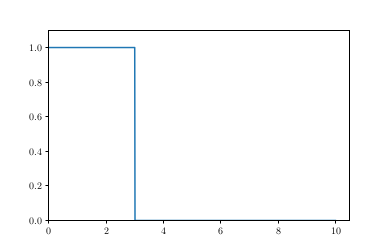
\includegraphics[width=0.8\linewidth]{images/crispFuzzifier.png}
	\captionof{figure}{Grafico esemplificativo di un crisp fuzzifier}
\end{minipage}

\item \emph{Linear Fuzzifier}: corrisponde a un fuzzy set la cui membership decresce linearmente da 1 a 0;


\begin{minipage}{\linewidth}
	\centering
      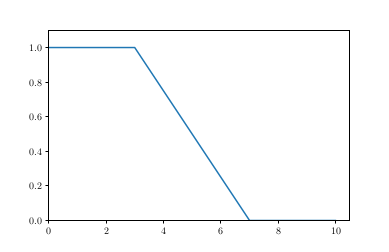
\includegraphics[width=0.8\linewidth]{images/linearFuzzifier.png}
	\captionof{figure}{Grafico esemplificativo di un linear fuzzifier}
\end{minipage}

\item \emph{Exponential Fuzzifier}: corrisponde a un fuzzy set la cui  membership diminuisce da 1 a 0 in maniera esponenziale. Il parametro $\alpha$ indica il decadimento esponenziale fissato;

\begin{minipage}{\linewidth}
	\centering
       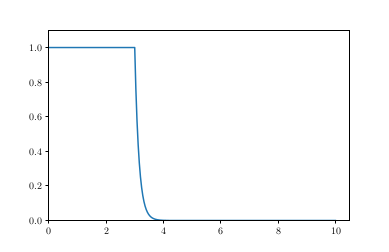
\includegraphics[width=0.8\linewidth]{images/exponentialFuzzifier.png}
	 \captionof{figure}{Grafico esemplificativo di un exponential fuzzifier con $\alpha$ = 0.001}
\end{minipage}

\begin{minipage}{\linewidth}
	\centering
       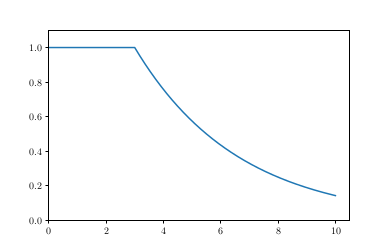
\includegraphics[width=0.8\linewidth]{images/exponentialFuzzifier2.png}
	 \captionof{figure}{Grafico esemplificativo di un exponential fuzzifier con $\alpha$  = 0.5}
\end{minipage}

\item \emph{Quantile Constant Piecewise Fuzzifier}:  corrisponde a un fuzzy set che ha una funzione di membership costante a tratti, per la quale gli step sono definiti in base ai quartili delle distanze al quadrato tra le immagini dei punti e il centro della sfera inferita; 

\begin{minipage}{\linewidth}
	\centering
       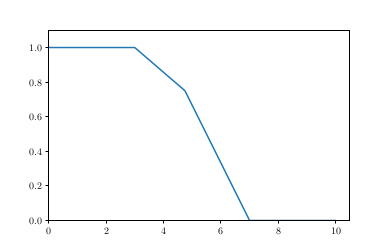
\includegraphics[width=0.8\linewidth]{images/quantileConstantPiecewiseFuzzifier.png}
	 \captionof{figure}{Grafico esemplificativo di un quantile constant piecewise fuzzifier}
\end{minipage}

\item \emph{Quantile Linear Piecewise Fuzzifier}:  corrisponde a un fuzzy set che ha una funzione di membership lineare a tratti, per la quale gli step sono definiti in base ai quartili delle distanze al quadrato tra le immagini dei punti e il centro della sfera inferita.

\begin{minipage}{\linewidth}
	\centering
       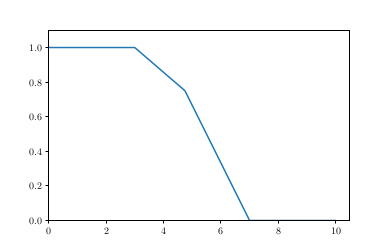
\includegraphics[width=0.8\linewidth]{images/quantileLinearPiecewiseFuzzifier.png}
	 \captionof{figure}{Grafico esemplificativo di un quantile linear piecewise fuzzifier}
\end{minipage}

\end{itemize}

Nella costruzione del FuzzyInductor si può optare per due tipi diversi di solver che risolvano il problema di ottimizzazione: il solver basato su Gurobi e quello basato su TensorFlow. 

Gurobi\cite{gurobi} è un solutore commerciale di ottimizzazione fondato nel 2008. Risolve problemi di programmazione lineare (LP), quadratica (QP), quadratica con vincoli (CQP), programmazione lineare intera mista (MILP), programmazione intera quadratica mista (MIQP) e programmazione intera quadratica con vincoli (MIQCP).

TensorFlow\cite{tensorFlow} è una piattaforma end-to-end open source per il machine learning. Viene utilizzata in ambiti di produzione e di ricerca scientifica, principalmente allo scopo di realizzare algoritmi per compiti percettivi e di comprensione del linguaggio.

\section{Il Kernel}\label{kernelSection}
Il parametro kernel della classe FuzzyInductor definisce quale sarà la funzione attraverso cui i valori verranno mappati nello spazio a più dimensioni.
La libreria mulearn implementa i seguenti kernel:

\begin{itemize}
\item \emph{Kernel lineare}: il valore $k(x_1,x_2)$ equivale al prodotto $x_1\cdot x_2$, ovvero  $\sum_{i=1}^N(x_1)_i\cdot(x_2)_i$, dove $N$ è la dimensione dei vettori $x_1$ e $x_2$;
\item \emph{Kernel polinomiale}: il valore $k(x_1,x_2)$ equivale a $(x_1\cdot x_2 + 1)^d$, dove $d$ è il grado polinomiale del kernel;
\item \emph{Kernel polinomiale omogeneo}:  il valore  $k(x_1,x_2)$ equivale a $(x_1\cdot x_2)^d$;
\item \emph{Kernel Gaussiano}:   il valore  $k(x_1,x_2)$ equivale a $e^{-\frac{||x_1 - x_2||^2}{2 \sigma^2}}$, dove $\sigma$ è la deviazione standard del kernel;
\item \emph{Kernel iperbolico}:   il valore $k(x_1,x_2)$  equivale a $\tanh(\alpha x_1 \cdot x_2 + \beta)$, dove $\alpha$ è la scala e $\beta$ l'offset.
\end{itemize}

La maggior parte dei kernel qui descritti richiedono di essere inizializzati con opportuni iper-parametri: nel capitolo \ref{capitoloEsperimenti} è stato esposto il procedimento di model selection effettuato su di essi.

\subsection{Kernel precomputato}
Per ottimizzare i tempi di computazione (i punti da mappare, nel caso di un insieme di formule, non corrispondono a valori numerici i cui valori del kernel sono semplici da calcolare) si è utilizzato un kernel precomputato, per il quale  $k(x_1,x_2)$ equivale a un valore precedentemente calcolato e salvato all'interno di una matrice, detta \emph{matrice di Gram}.
Per calcolarlo, ovvero trovare un criterio per definire il grado di similarità tra due assiomi, si utilizza un indice di similarità ispirato alla similarità di Jaccard, descritta in \cite{sacpaper}.
Per tutte le coppie di assiomi $\phi$ e $\psi$, la definizione di similarità deve rispettare le seguenti proprietà:
\begin{itemize}
\item $0 \leq sim(\psi, \phi) \leq 1$. Si sta infatti operando in un ambito possibilistico, nel quale a ogni assioma viene associato un grado di possibilità compreso tra 0 e 1;
\item $sim(\psi, \phi) = 1$ sse $\psi \equiv \phi $;
\item $sim(\psi, \phi) = sim(\phi,\psi)$.
\end{itemize}
Se si riuscisse a definire una funzione $Impl(\phi,\psi)$, allora si potrebbe dire $sim(\psi, \phi) = min\{Impl(\phi,\psi), Impl(\psi,\phi)\}$, dove il minimo traduce la congiunzione delle due condizioni logiche.
Per definire l'implicazione, ci si può avvalere della definizione classica di implicazione materiale, ovvero $Impl(\psi,\phi) = 1$ se $\models \lnot \phi \lor \psi$, 0 altrimenti.


Si può restringere il campo agli assiomi di inclusione di cui ci si è occupati nello specifico, ovvero formule del tipo \emph{Subclass(B,C)}, o 	$B \sqsubseteq C$ in forma più compatta, e le loro negazioni \emph{ $\lnot Subclass(B,C)$} e {$ B \not\sqsubseteq C$}.
Avendo a disposizione un insieme di assiomi, si può dire che $a$ conferma $B \sqsubseteq C$ ( e contraddice  {$ B \not\sqsubseteq C$}) se vale $B(a) \land C(a)$, $a$ contraddice  $B \sqsubseteq C$ (e conferma {$ B \not\sqsubseteq C$}) se vale $B(a) \land \lnot C(a)$.
Dunque, sfruttando la definizione precedentemente data di implicazione materiale, si può affermare:

\[Impl(A \sqsubseteq B, C \sqsubseteq D) = \frac{\parallel \{ a: (A(a) \land \lnot B(a)) \lor (C(a) \land D(a)) \} \parallel}{\parallel \{ a: (A(a) \lor C(a))\} \parallel}. \]

Se si definisce

\[ [C] = \{a : C(a) \},\]

allora si può scrivere la formula precedente come:

\[ \frac{\parallel [A] \cup [\overline{B}] \cup [C] \cap [D] \parallel}{\parallel [A] \cup [C] \parallel}.\]

Avendo precedentemente definito l'operatore di similarità tra due assiomi in relazione al minimo tra le due implicazioni, risulta:

\[ sim(A \sqsubseteq B, C  \sqsubseteq D) = min\{Impl(A \sqsubseteq B, C\sqsubseteq D), Impl( C\sqsubseteq D, A \sqsubseteq B)\} \]
\[ = min\bigg\{\frac{\parallel [A] \cap [\overline{B}] \cup [C] \cap [D] \parallel}{\parallel [A] \cup [C] \parallel}, \frac{\parallel [C] \cup [\overline{D}] \cup [C] \cap [D] \parallel}{\parallel [A] \cup [C] \parallel}\bigg\}.\]
\[ = \frac{min\{\parallel [A] \cap [\overline{B}] \cup [C] \cap [D] \parallel, \parallel [C] \cup [\overline{D}] \cup [C] \cap [D] \parallel\}}{\parallel [A] \cup [C] \parallel}.\]

Nella pratica, per calcolare i valori del kernel precomputato si è utilizzata una versione semplificata della formula precedente, ovvero:

\[sim(A \sqsubseteq B, C  \sqsubseteq D) = \frac{\parallel [A] \cap [B] \cup [C] \cap [D] \parallel}{\parallel [A] \cup [C] \parallel}. \]

Utilizzando questa definizione di similarità, i risultati ottenuti in termini di RMSE per i valori di test e per i valori di train sono riportati nella tabella ~\ref{table:risultatiJaccard}.

\begin{table}
\small
\centering 	
	\begin{tabular}{|c|c|c|}
	 \hline
	  & RMSE test(+/- std) & RMSE train (+/- std)\\ [0.5ex] 
	 \hline
	 Crisp Fuzzifier & 0.26974 +/ 0.27 & 0.21694 +/- 0.024 \\ 
	 \hline
	 Quantile Constant Piecewise Fuzzifier & 0.11759 +/- 0.108 & 0.10881 +/- 0.02\\
	 \hline
	 Quantile Linear Piecewise Fuzzifier & 0.1032 +/- 0.08 & 0.09935 +/- 0.014\\
	 \hline
	 Linear Fuzzifier & 0.15256 +/- 0.172 & 0.13883 +/- 0.024\\
	 \hline
	 Exponential Fuzzifier & 0.13603 +/- 0.17 & 0.13391 +/- 0.02\\ [1ex] 
	 \hline
	\end{tabular}
\caption{Valori ottenuti con la similarità di Jaccard}
\label{table:risultatiJaccard}
\end{table}

\subsection{Kernel alternativi}
Nel corso degli esperimenti sono state utilizzate altre definizioni di similarità, diverse da quella di Jaccard, descritte in \cite{drtpaper}.
\subsubsection{Length-based similarity}
Una prima forma ingenua di similarità utilizzata è quella basata sulla lunghezza degli assiomi.
Si definisce dunque

\[ s_{len}(\phi_1, \phi_2) = 1 - \frac{|\# \phi_1 - \# \phi_2|}{max\{\#\phi_1, \#\phi_2\}},\]

ovvero il valore assoluto della differenza tra le due lunghezze, normalizzato.
Tale formulazione nasconde una problematica: quando un assioma è il negato dell'altro la funzione restituisce un valore di similarità alto. Occore, pertanto, introdurre un'ulteriore casistica: se i segni dei due assiomi sono diversi, la funzione di similarità vale $1 - s_{len}(\phi_1,\phi_2)$.
Una nuova classe kernel è stata implementata per essere utilizzata in modo da computare direttamente il valore di similarità basato su lunghezza dei due assiomi, senza passare per la creazione o il caricamento della matrice di Gram con i valori precalcolati.
Per velocità di computazione si è scelto di implementare solamente la prima versione della funzione, ignorando il problema del valore di similarità per assiomi opposti l'uno all'altro.
Anche agendo in questo modo, il tempo di computazione è risultato accettabile per un massimo di 50 assiomi su 1444; si è scelto, pertanto, di utilizzare matrice e kernel precomputato anche per questa definizione di similarità. La tabella \ref{table:risultatiLength} mostra i risultati ottenuti. L'ingenuità del metodo faceva supporre un generale peggioramento dei risultati rispetto alla similarità di Jaccard, che anzi si presupponeva più consistente di quello effettivamente riscontrato.

\begin{table}[h!]
\small
\centering 	
	\begin{tabular}{|c|c|c|} 
	 \hline
	  & RMSE test(+/- std) & RMSE train (+/- std)\\ [0.5ex] 
	 \hline
	 Crisp Fuzzifier & 0.38573 +/- 0.466 & 0.391 +/- 0.108 \\ 
	 \hline
	 Quantile Constant Piecewise Fuzzifier & 0.31572 +/- 0.288 & 0.31 +/- 0.058\\
	 \hline
	 Quantile Linear Piecewise Fuzzifier & 0.30646 +/- 0.252 & 0.3 +/- 0.052\\
	 \hline
	 Linear Fuzzifier & 0.24792 +/- 0.092 & 0.225 +/- 0.014\\
	 \hline
	 Exponential Fuzzifier & 0.24521 +/- 0.11 & 0.224 +/- 0.014\\ [1ex] 
	 \hline
	\end{tabular}
	\caption{Valori ottenuti con Length Similarity}	
	\label{table:risultatiLength}
\end{table}

\subsubsection{Hamming similarity}
Altro modo di definire la similarità tra due assiomi è la distanza di Hamming, ovvero la distanza tra le rappresentazioni testuali delle due formule, intesa come il numero di caratteri diversi tra una e l'altra, trascurando i caratteri extra della stringa più lunga.
Definendo H la distanza di Hamming, si fa la stessa distinzione descritta precedentemente per gli assiomi di segno opposto:  $sim_{H}(\phi_1, \phi_2) = H(abs(\phi_1),abs(\phi_2))$ se i segni delle due formule sono opposti, $1 - H(\phi_1, \phi_2)$ altrimenti.
Anche in questo caso, l'implementazione della classe \emph{HammingKernel} non ha portato ai risultati sperati, a causa dell'eccessivo costo computazionale di calcolare la distanza di Hamming per ognuno dei 1444 assiomi. Gli esperimenti con la matrice di Gram hanno invece condotto ai risultati riportati nella tabella \ref{table:risultatiHamming}. I valori di RMSE e varianza risultano complessivamente peggiori rispetto alla similarità di Jaccard, e stranamente non molto migliori di quelli basati sulla lunghezza: anzi, utilizzando il CrispFuzzifier risultano essere perfino peggiori di questi ultimi.

\begin{table}[h!]
\small
\centering 	
	\begin{tabular}{|c|c|c|} 
	 \hline
	  & RMSE test(+/- std) & RMSE train (+/- std)\\ [0.5ex] 
	 \hline
	 Crisp Fuzzifier & 0.54868 +/- 0.418 & 0.713 +/- 0.118 \\ 
	 \hline
	 Quantile Constant Piecewise Fuzzifier & 0.35935 +/- 0.198 & 0.448 +/- 0.064\\
	 \hline
	 Quantile Linear Piecewise Fuzzifier & 0.35008 +/- 0.162 & 0.42 +/- 0.06\\
	 \hline
	 Linear Fuzzifier &0.23933 +/- 0.11 & 0.191 +/- 0.066\\
	 \hline
	 Exponential Fuzzifier & 0.22399 +/- 0.088 & 0.198 +/- 0.016\\ [1ex] 
	 \hline
	\end{tabular}
	\caption{Valori ottenuti con la similarità di Hamming}
	\label{table:risultatiHamming}
\end{table}

\subsubsection{Levenshtein similarity}
L'ultima funzione di similarità utilizzata è la distanza di Levenshtein tra due stringhe, ovvero il numero più piccolo di operazioni atomiche che vanno fatte per trasformare una nell'altra. Chiamando questa funzione \emph{Lev}, $sim_{edit}(\phi_1, \phi_2) = 1 - Lev(\phi_1,\phi_2)$ se i due segni sono diversi, $Lev(abs(\phi_1),abs(\phi_2))$ altrimenti.
Come nei due casi precedenti, si è continuato a dover utilizzare una matrice di Gram precalcolata per definire i valori del kernel in un tempo accettabile. I valori dell'RMSE ottenuti sono mostrati nella tabella \ref{table:risultatiLevenshtein} e risultano valere le stesse considerazioni fatte per la distanza di Hamming.

\begin{table}[h!]
\small
\centering 	
	\begin{tabular}{|c|c|c|} 
	 \hline
	  & RMSE test(+/- std) & RMSE train (+/- std)\\ [0.5ex] 
	 \hline
	 Crisp Fuzzifier & 0.50254 +/- 0.388 & 0.73 +/- 0.076 \\ 
	 \hline
	 Quantile Constant Piecewise Fuzzifier & 0.36324 +/- 0.122 & 0.439 +/- 0.058\\
	 \hline
	 Quantile Linear Piecewise Fuzzifier & 0.35503 +/- 0.138	 & 0.412 +/- 0.05\\
	 \hline
	 Linear Fuzzifier & 0.23958 +/- 0.094 & 0.201 +/- 0.068\\
	 \hline
	 Exponential Fuzzifier & 0.23807 +/- 0.11 & 0.198 +/- 0.07\\ [1ex] 
	 \hline
	\end{tabular}
	\caption{Valori ottenuti con la similarità di Levenshtein}
	\label{table:risultatiLevenshtein}
\end{table}


\chapter{Esperimenti}\label{capitoloEsperimenti}
Qui andrei a mostrare gli esperimenti e i relativi risultati conseguiti tramite cross validation e model selection.
\section{Riproduzione degli esperimenti originali}
\section{Esperimenti sul kernel}
\subsection{Kernel alternativi}
\subsection{Possibili soluzioni al problema del fitting}
\subsubsection{Eliminazione combinatoria di formule}
\subsubsection{Eliminazione a campione di formule}
\subsubsection{Valori di similarità come vettori in input all'algoritmo}

\chapter*{Conclusione}

\bibliographystyle{plain}
\bibliography{Biblio}
%\addcontentsline{toc}{chapter}{Bibliografia}

\end{document}
